\subsubsection{Bayesian reweighting analysis}

The procedure followed to quantify the impact of future
lattice QCD calculations
in PDF fits  (for the three scenarios of Table~\ref{tab:scenarios})
is common for unpolarized
and polarized global analyses.
%
We briefly describe this procedure here,
and refer to~\cite{Ball:2011gg,Ball:2010gb} for
additional details.
\begin{itemize}
\item First of all, we generate pseudo-data for the lattice QCD calculation
  of the PDF moments used in this exercise, namely $\la x\ra_{u^+}$,
$\la x\ra_{d^+}$,
$\la x\ra_{s^+}$,
$\la x\ra_{g}$, and
  $\la x\ra_{u^+-d^+}$ for the unpolarized case, and
  $\la 1\ra_{\Delta u^+}$,
$\la 1\ra_{\Delta d^+}$,
$\la 1\ra_{\Delta s^+}$,
$\la x\ra_{\Delta u^--\Delta d^-}$, and
  $\la 1\ra_{\Delta u^+ - \Delta d^+}$ for the polarized case.
  %
  We denote generically these moments by $\mathcal{F}_i$.
\item This pseudo-data, denoted by $\mathcal{F}_i^{\rm (exp)}$,
  is constructed by taking the central values from
  the corresponding NNPDF fits, NNPDF3.1 NNLO for the unpolarized case and NNPDFpol1.1 NLO
  for the polarized one.
  %
  That is, we {\it assume} for simplicity that the central value
  of such future lattice calculations would coincide with the current ones
  from the global fit.\footnote{Repeating the exercise with the actual lattice QCD
    central values would be straightforward, but
    lies beyond the scope of the present studies.}
  %
  As discussed in Sect.~\ref{sec:unpPDFs}, this corresponds to computing
  the mean over the Monte Carlo replica sample,
  \be
  \label{eq:pseudodatadef}
  \mathcal{F}_i^{\rm (exp)} \equiv \frac{1}{N_{\rm rep}}\sum_{k=1}^{N_{\rm rep}}
  \mathcal{F}_i^{\rm (k)} \, , \quad i=1,\ldots,N_{\rm mom} \, ,
  \ee
  where $N_{\rm mom}$ are the number of PDF moments that will be included
  in the reweighting, in this case $N_{\rm mom}=5$ both for the unpolarized
  and polarized cases.
  %
  To be consistent with the calculations in Sect.~\ref{sec:benchmarking},
  here the central values of the pseudo-data Eq.~(\ref{eq:pseudodatadef})
  are also evaluated at $Q^2=4$ GeV$^2$ (see Tables~\ref{tab:unpPDFmoms} and~\ref{tab:polPDFmoms}).
\item The uncertainty in the pseudo data, denoted by $\delta\mathcal{F}_i^{\rm (exp)} $,
  is taken for each moment to be the value indicated in
  Table~\ref{tab:scenarios} for each of the three scenarios.%
  That is, we have that the absolute uncertainty on the $i$-th moment
  will be given by $\delta\mathcal{F}_i^{\rm (exp)}=\delta_L^{(i)}\mathcal{F}_i^{\rm (exp)} $.
\item Using the pseudo-data (central values and total uncertainties)
  as defined above, we next need to compute
  the weights  $\omega_k$.
  %
  These weights
  quantify the agreement between each of $N_{\rm rep}$ replicas
  of the input PDF set and the corresponding lattice pseudo-data.
  %
  Specifically, first of all we compute the $\chi^2$ between each of the Monte Carlo
  replicas and the lattice pseudo-data as follows,
  \be
  \chi^{2(k)}= \sum_{i=1}^{\rm N_{\rm mom}} \frac{\lp
    \mathcal{F}_i^{\rm (k)} -\mathcal{F}_i^{\rm (exp)} \rp^2}{
    \lp \delta\mathcal{F}_i^{\rm (exp)}\rp^2} \, , \quad k=1,\ldots,N_{\rm rep} \, ,
  \ee
  assuming that there are no correlations between the different $N_{\rm mom}$ moments.
  %
  This assumption in general might not be a good approximation, since most lattice
  QCD systematic errors are correlated among the different moments, and should be
  avoided provided the full breakdown of systematic error of each quantity is available.

  
  Once the values of the $\chi^2$ have been evaluated,
  we can compute the corresponding weights for each replica.
  %
  The relation between the weights $w_k$  and the values of
  the $\chi^{2(k)}$ of each replica is the following
  \be
  \omega_k =\frac{\lp \chi^{2(k)} \rp^{(N_{\rm mom}-1)/2}\exp(-\chi^{2(k)}/2)}{
  \sum_{k=1}^{N_{\rm rep}} \lc \lp \chi^{2(k)} \rp^{(N_{\rm mom}-1)/2}\exp(-\chi^{2(k)}/2)\rc} \, ,
  \ee
  where the denominator ensures that the weight admit
  a probabilistic interpretation, that is, $\sum_k w_k=1$.
  %
  These weights represent a measure of the agreement of the individual replicas with the new pseudo-data.
  %
  For instance, replicas which have associated values
  of the moments far from the pseudo-data (within uncertainties) will
  have associated a very large weight, being thus effectively discarded.
\item These weights can be use to now recompute the PDFs, their moments,
  as well as any generic cross-section.
  %
  This procedure emulates the
  impact that adding these lattice-QCD pseudo-data in a complete PDF fit would have.
  %
  For instance, after the reweighting the mean value of
  the PDF moments should be computed as
   \be
  \label{eq:pseudodatadef1}
  \mathcal{F}_i^{\rm (rw)} \equiv \frac{1}{N_{\rm rep}}\sum_{k=1}^{N_{\rm rep}}\omega_k
  \mathcal{F}_i^{\rm (k)} \, , \quad i=1,\ldots,N_{\rm mom} \, ,
  \ee
  and same for the associated uncertainties.
\end{itemize}

One limitation of the reweighting procedure just
outlined is that it can be considered as fully 
 reliable provided only the 
  effective number of replicas $N_{\rm eff}$ that survive the reweighting
  procedure (which is a measure of the amount
  of information left) is not too small.
  %
  This effective number of replicas
    is quantified in terms of the Shannon entropy from information
    theory, namely
    \be
    \label{eq:effnrep}
    N_{\rm eff}\equiv \exp\lc \frac{1}{N_{\rm rep}}\omega_k
    \log \lp N_{\rm rep}/\omega_k\rp\rc \, .
    \ee
    Finding that $N_{\rm eff}\ll N_{\rm rep}$ means that the pseudo-data
    has a large impact on the fit, potentially leading to a large
    reduction of the PDF uncertainties.
    %
    But if the effective number of replicas becomes too
    small, say $N_{\rm eff}\lsim 25$, then the results
    become unreliable since they are affected by large
    statistical fluctuations.

    Therefore, before considering the effects
    of the lattice-QCD pseudo-data at the PDF
    level, we need to ensure that the
    three scenarios defined
    in Table~\ref{tab:scenarios} still lead
    to values of $N_{\rm eff}$ large enough for
    the reweighting procedure to be reliable.
  %
In Table~\ref{tab:neff} we indicate the effective number of replicas
    $N_{\rm eff}$, Eq.~(\ref{eq:effnrep}), remaining when the pseudo-data
    on the PDF moments is included in the global
    fit according to the 
    %
    For completeness, we also indicate here the original number
    of replicas $N_{\rm rep}$ for the original
    PDF sets, NNPDF3.1 NNLO and NNPDFpol1.1 respectively.
    %
    As we can see, there is a marked decrease of $N_{\rm rep}$
    for the three scenarios, indicating that adding the
    PDF moments leads to non-trivial constraints on the global
    fit.
    %
    For instance, in the most optimistic scenario,
    Scenario A, the effective number of replicas is around five (three)
    smaller than the starting number of replicas.

%%%%%%%%%%%%%%%%%%%%%%%%%%%%%%%%%%%%%%%%%%%%%%
\begin{table}[t]
  \centering
  \renewcommand{\arraystretch}{1.3} 
  \begin{tabular}{c|c|c}
    \hline
    &  NNPDF3.1  &  NNPDFpol1.1 \\
    \hline
    \hline
    $N_{\rm rep}$ original   &   1000 &  100   \\
    \hline
     $N_{\rm eff}$ Scenario A    &   740  &  72   \\
     $N_{\rm eff}$ Scenario B    &   750   &   59  \\
     $N_{\rm eff}$ Scenario C   &   510  &   20  \\
    \hline
  \end{tabular}
  \caption{\small The effective number of replicas
    $N_{\rm eff}$, Eq.~(\ref{eq:effnrep}), remaining when the pseudo-data
    on the PDF moments is included in the global
    fit according to the scenarios outlined
    in Table~\ref{tab:scenarios}.
    %
    For completeness, we also indicate the original number
    of replicas $N_{\rm rep}$ for the original
    PDF sets, NNPDF3.1 NNLO and NNPDFpol1.1 respectively.
    \label{tab:neff}
  }
\end{table}
%%%%%%%%%%%%%%%%%%%%%%%%%%%%%%%%%%%%%%%%%%%%%%

\subsubsection*{Impact on unpolarized global fits}
\label{subsec:upolfits}
%
We start by discussing the results of applying the reweighting procedure
outlined above to a representative unpolarized
global fit, in this case the NNPDF3.1 NNLO analysis.
%
To begin with, in Table~\ref{tab:unpolmomentsrw} we summarize
the values of the unpolarized PDF moments
used as pseudo-data $\mathcal{F}_i^{(\rm exp)}$,
as well as the corresponding results
  after the reweighting has been performed for the
three scenarios summarized in 
in Table~\ref{tab:scenarios}.
%
The PDF uncertainties quoted there correspond to 68\% confidence level intervals.
%
We recall that, as explained above, the three scenarios considered here exhibit
uncertainties $\delta_L^{(i)}$ on the lattice-QCD pseudo-data rather smaller
than those of current calculations (see Table~\ref{tab:BMunp}).

%%%%%%%%%%%%%%%%%%%%%%%%%%%%%%%%%%%%%%%%%%%%%%%%%%%%%%%%
\begin{table}[t]
  \centering
  \renewcommand{\arraystretch}{1.3} 
\begin{tabular}{c||c|c|c|c}
  \hline &  Original  & Scen A  &  Scen B  &  Scen C  \\
  \hline
  \hline
  $\la x\ra_{u^+}$     &   $0.348 \pm  0.005$    &  $ 0.349 \pm 0.004$     &
  $ 0.349 \pm 0.004$   &  $ 0.349 \pm 0.003$   \\
  $\la x\ra_{d^+}$     &   $0.196\pm  0.004$     & $0.196 \pm0.004$       &
  $0.196 \pm0.003$ &   $0.196 \pm0.002$ \\
  $\la x\ra_{s^+}$     &   $0.0393 \pm 0.0036$   &  $0.0389\pm 0.0030$   &
 $0.0389\pm 0.0024$   &   $0.0389\pm 0.0014$  \\
  $\la x\ra_{g}$       &   $0.4097\pm 0.0042$    &  $0.4097 \pm 0.0043$    &
   $0.4097 \pm 0.0040$  &    $0.4097 \pm 0.0029$  \\
  $\la x\ra_{u^+-d^+}$  &   $0.1522 \pm 0.0033$   &  $0.1521 \pm 0.0037$   &
   $0.1521 \pm 0.0035$ &    $0.1521 \pm 0.0029$ \\
  \hline
\end{tabular}
\caption{\small Values of the unpolarized PDF moments
  used as pseudo-data, as well as the corresponding results
  after the reweighting has been performed for the
three scenarios summarized in 
in Table~\ref{tab:scenarios}.
%
The PDF uncertainties quoted correspond in all cases to 68\%
CL intervals.
\label{tab:unpolmomentsrw}
}
\end{table}
%%%%%%%%%%%%%%%%%%%%%%%%%%%%%%%%%%%%%%%%%%%%%%%%%%%%%%%%

From Table~\ref{tab:unpolmomentsrw} we see that a significant
reduction of the uncertainties in the unpolarized PDF moments is challenging to achieve
unless we go to the most aggressive scenarios.
%
For instance, in scenario C, which is about the best precision that
can achieved from lattice-QCD, the PDF uncertainties on the second moments
(that is, the momentum fractions) for $u^+,d^+,s^+$ and $g$ decrease by around
between 30\% and 60\%.
%
The most marked decrease is for the strange momentum fraction, since this is the
one affected by the largest PDF errors to begin with.
%
On the other hand, the non-singlet combination $\la x\ra_{u^+-d^+}$ is essentially
unchanged in all three scenarios.
%
Note that the reason why in Table~\ref{tab:unpolmomentsrw} the central values
of the PDF moments are very stable is that by construction we assume that the
lattice-QCD central value corresponds to the PDF one.
%
Of course in a realistic situation, such as that summarized in the
comparisons of Fig.~\ref{fig:Bmoms}, this will not be necessarily the case
and there also the central value of the PDF moments expected to vary
upon reweighting.


%------------------------------------------------------
\begin{figure}[!t]
\centering
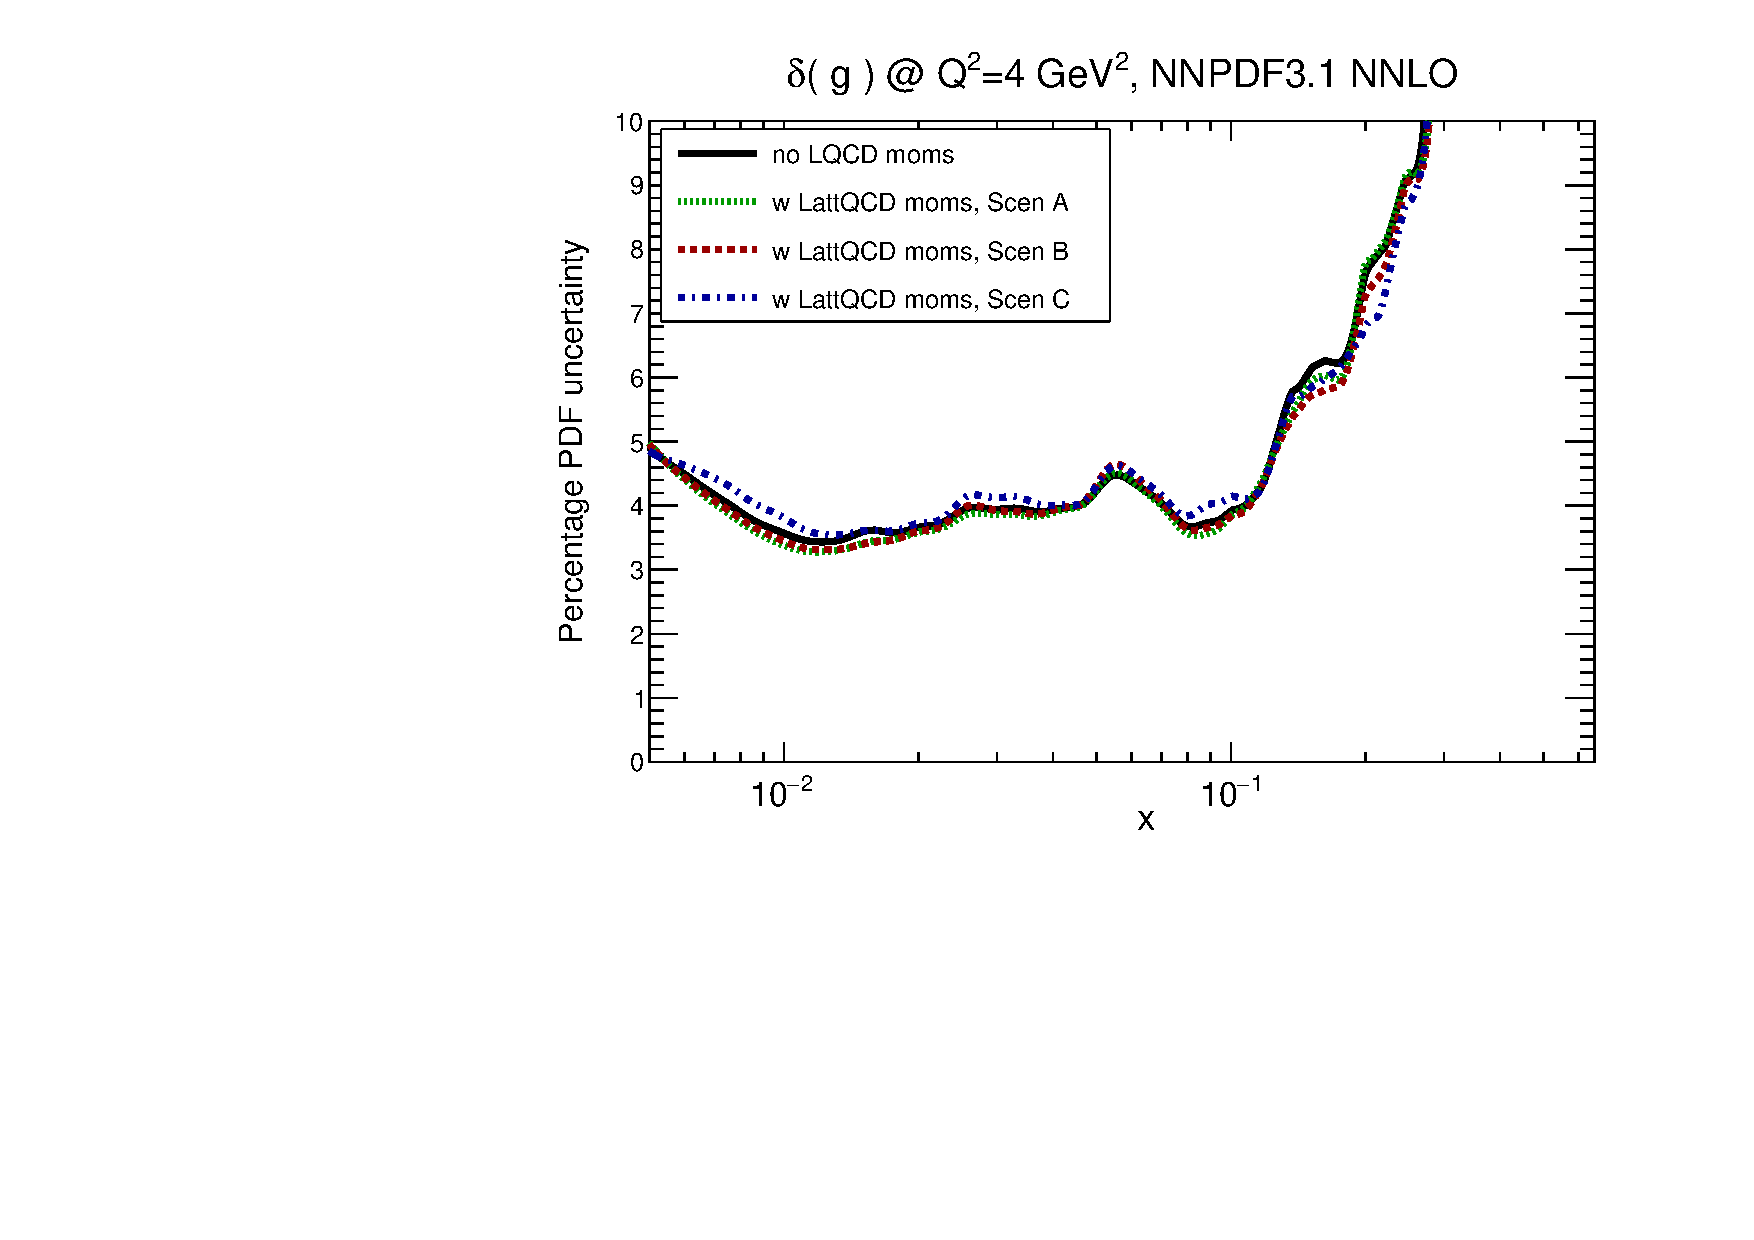
\includegraphics[scale=0.45]{plots/xg-unpol-lattice-relerr.pdf}
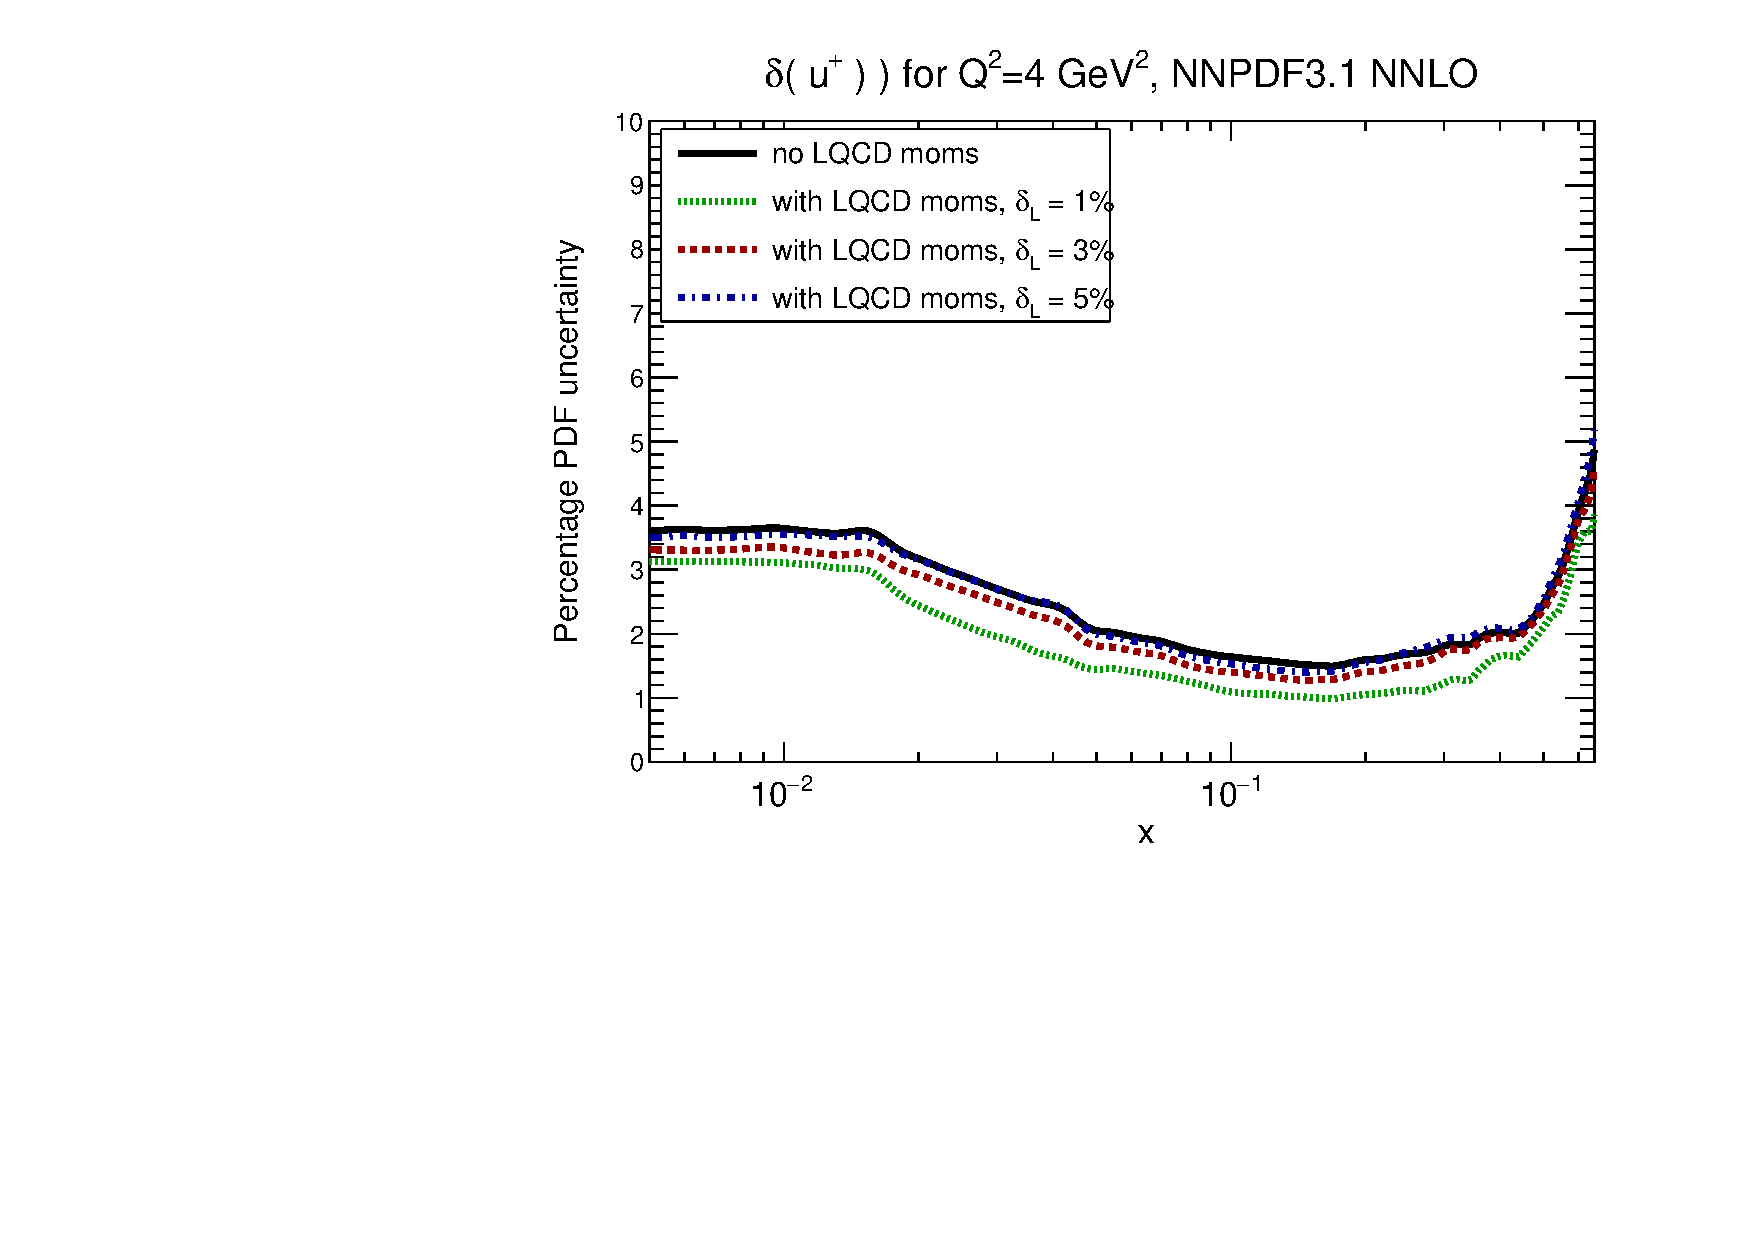
\includegraphics[scale=0.45]{plots/xup-unpol-lattice-relerr.pdf}
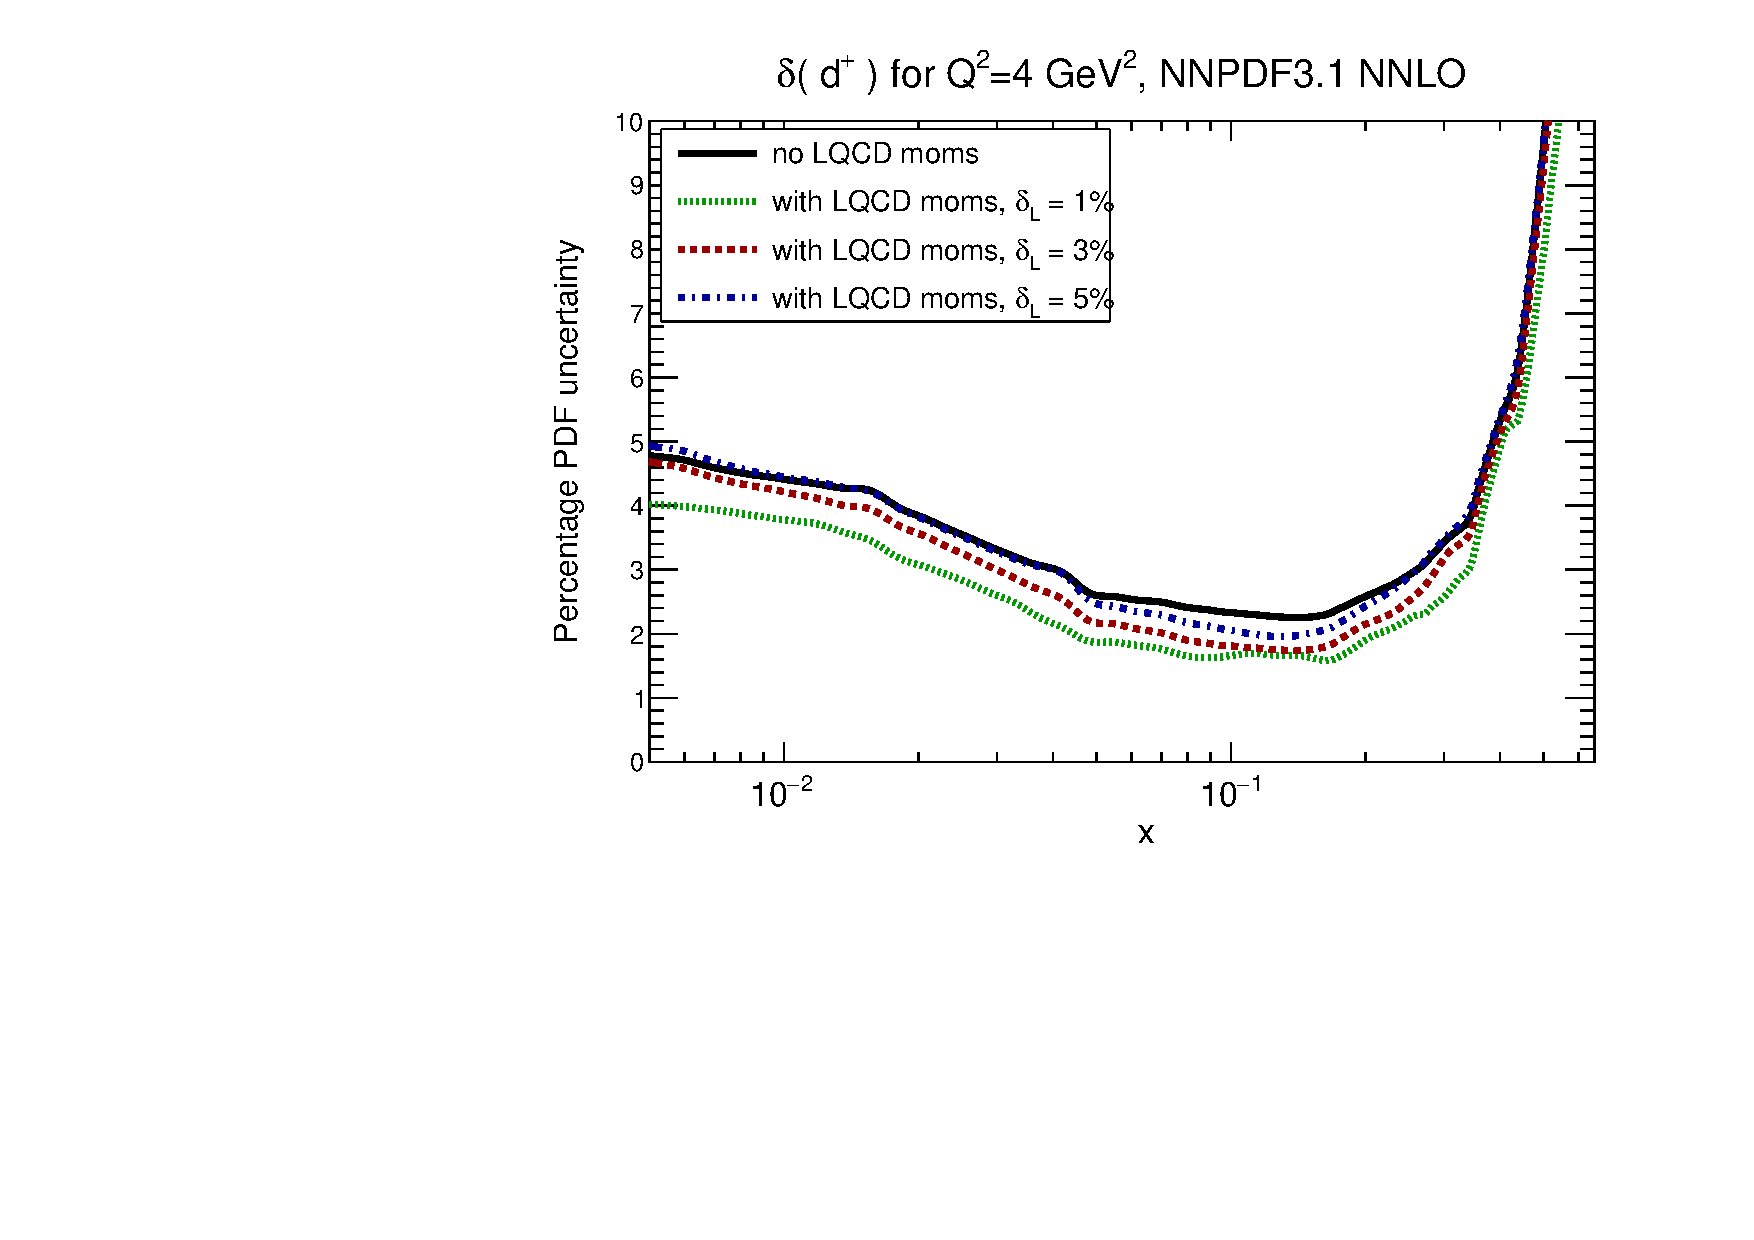
\includegraphics[scale=0.45]{plots/xdp-unpol-lattice-relerr.pdf}
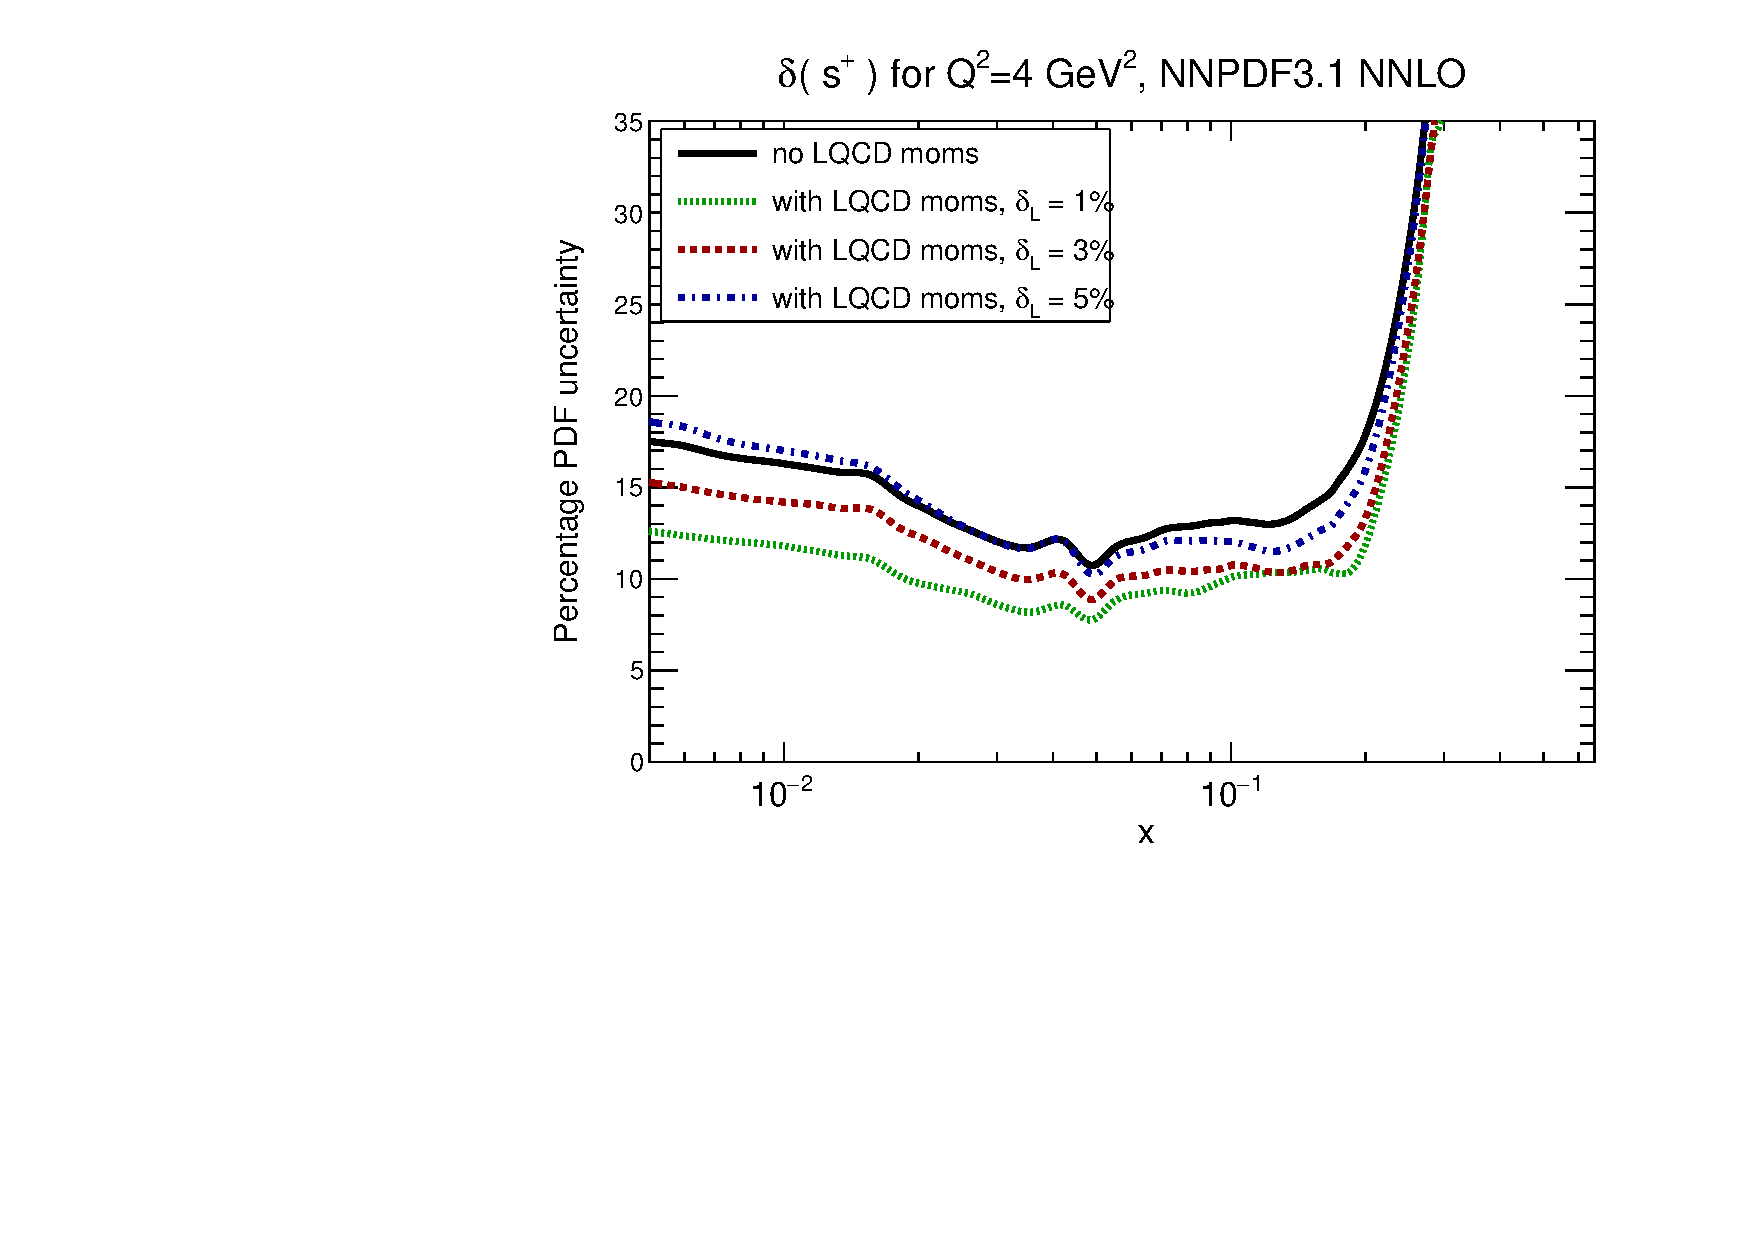
\includegraphics[scale=0.45]{plots/xsp-unpol-lattice-relerr.pdf}
\caption{\small The percentage PDF uncertainty in NNPDF3.1 NNLO
  for the gluon and the $u^+$, $d^+$ and $s^+$ quark PDFs at
  $Q^2=4$ GeV$^2$,
  compared to the results of including the five lattice
  QCD moments as pseudo-data points in the fit using the three
  different scenarios in  Table~\ref{tab:scenarios}.
  %
See text for more details.
}    
\label{fig:impactUnpol}
\end{figure}
%----------------------------------------------------------

The result that, at least with the specific moments that we have used
in this exercise, it will be challenging to reduce the
PDF uncertainties is also illustrated by the comparisons of 
 Fig.~\ref{fig:impactUnpol}, where we show
percentage PDF uncertainty in NNPDF3.1 NNLO
for the gluon and the $u^+$, $d^+$ and $s^+$ quark PDFs in NNPDF3.1 NNLO
at $Q^2=4$ GeV$^2$,
compared to the corresponding results once
the lattice-QCD pseudo-data points of Table~\ref{tab:scenarios} have
been added by reweighting.
  %
In the case of the $u^+,d^+$ and $s^+$, we observe a slight reduction
of the PDF uncertainties, which is more marked as the move
from scenario A to C.
%
For instance, in the latter case the percentage PDF
uncertainty on $u^+$ ($d^+$ and $s^+$) at $x\simeq 0.1$
decreases from 1.8\% to 1.2\% (from 2.2\% to 1.7\% and from 13\% to 10\% respectively).
%
The PDF uncertainties of the gluon PDF, however,
are essentially unchanged even in the most optimistic scenario.

Focusing on the large-$x$ region, where the sensitivity to the
results of the second moments is more marked, in
Fig.~\ref{fig:impactUnpollargex} we show a similar comparison
as in Fig.~\ref{fig:impactUnpo} but now showing the ratio of the
  PDF uncertainties in the fits based on the three scenarios
  as a ratio of the original
  PDF uncertainty of the NNPDF3.1 NNLO set, for the $d^+$
  and $s^+$ total quark PDFs.
  %
  This comparison illustrates better that the relative reduction
  of the PDF uncertainties upon the addition of the lattice-QCD
  pseudo-data is not completely flat, and that it exhibits some
  non-trivial structure.

%------------------------------------------------------
\begin{figure}[!t]
\centering
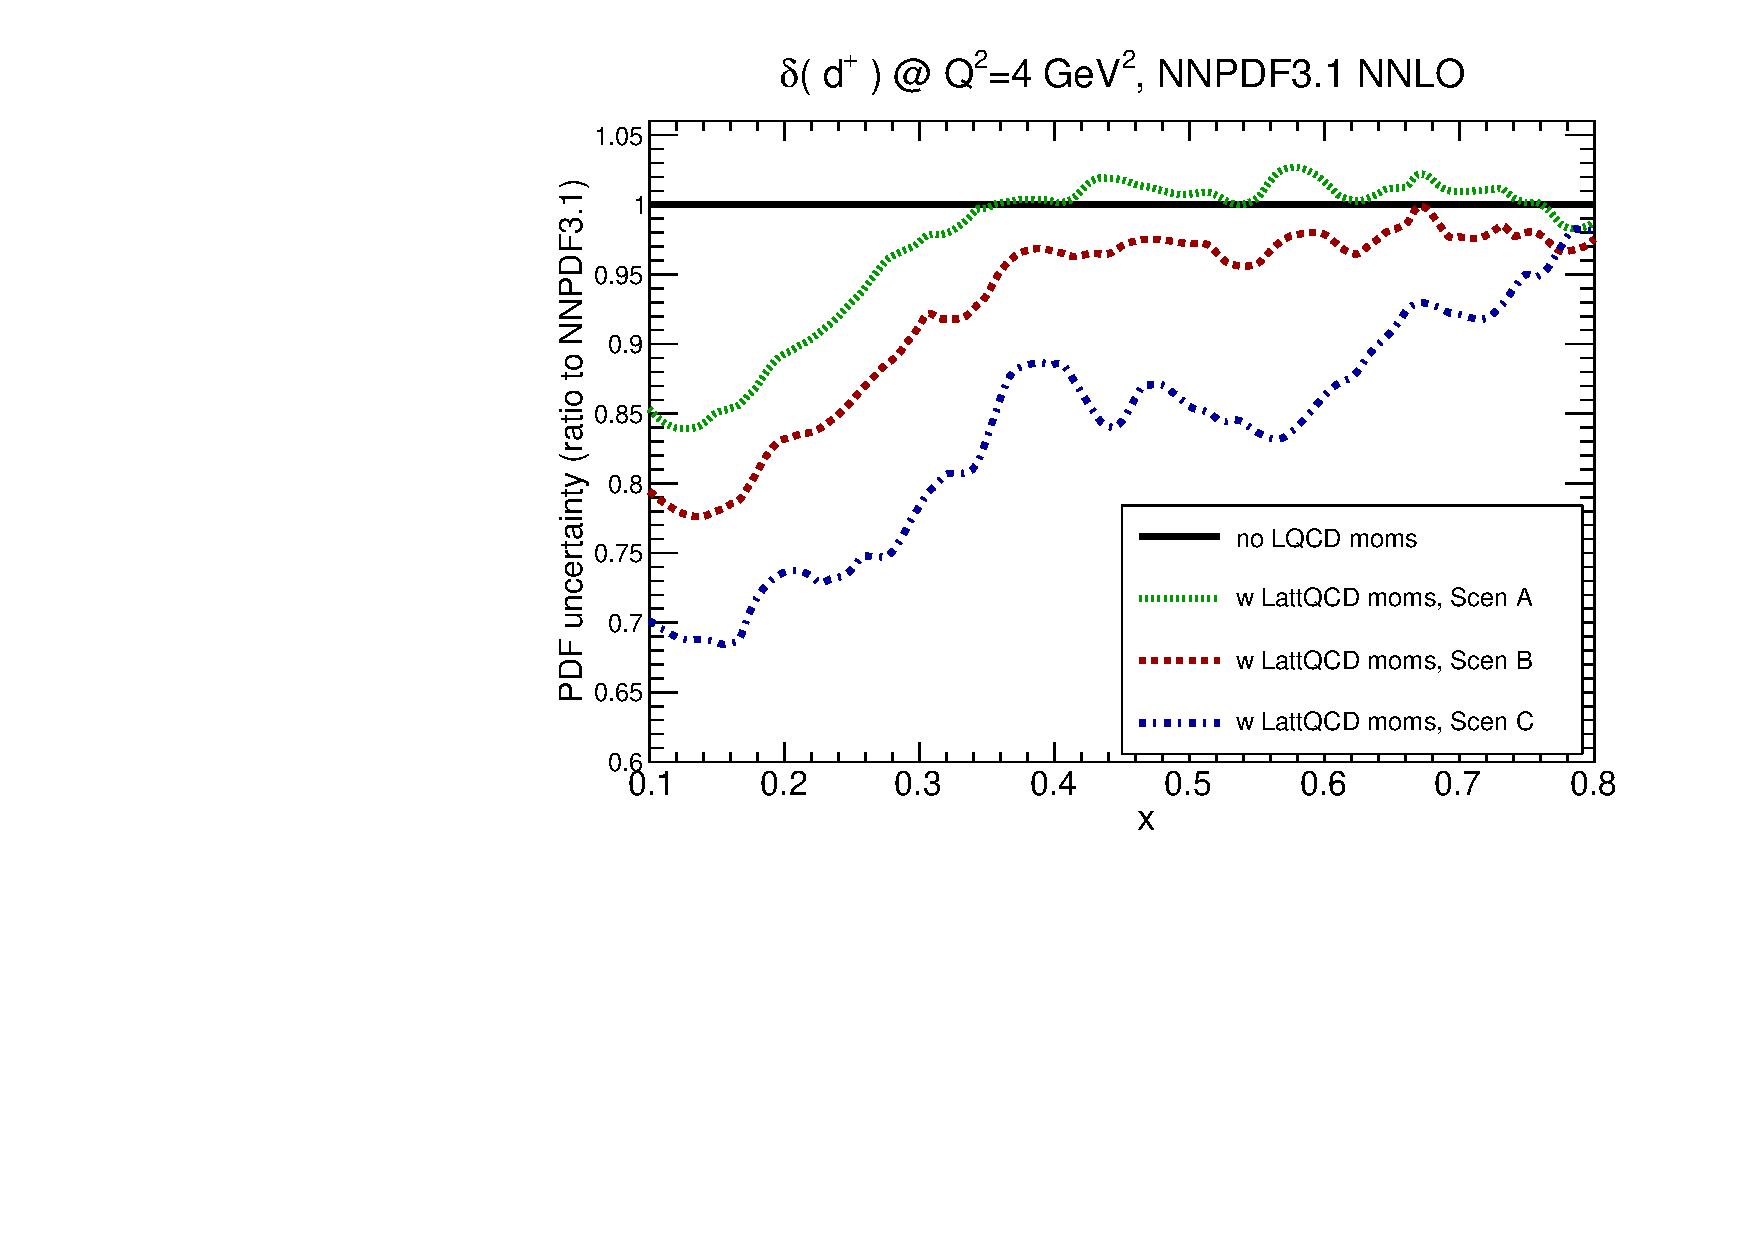
\includegraphics[scale=0.45]{plots/xdp-unpol-lattice-relerr-largex.pdf}
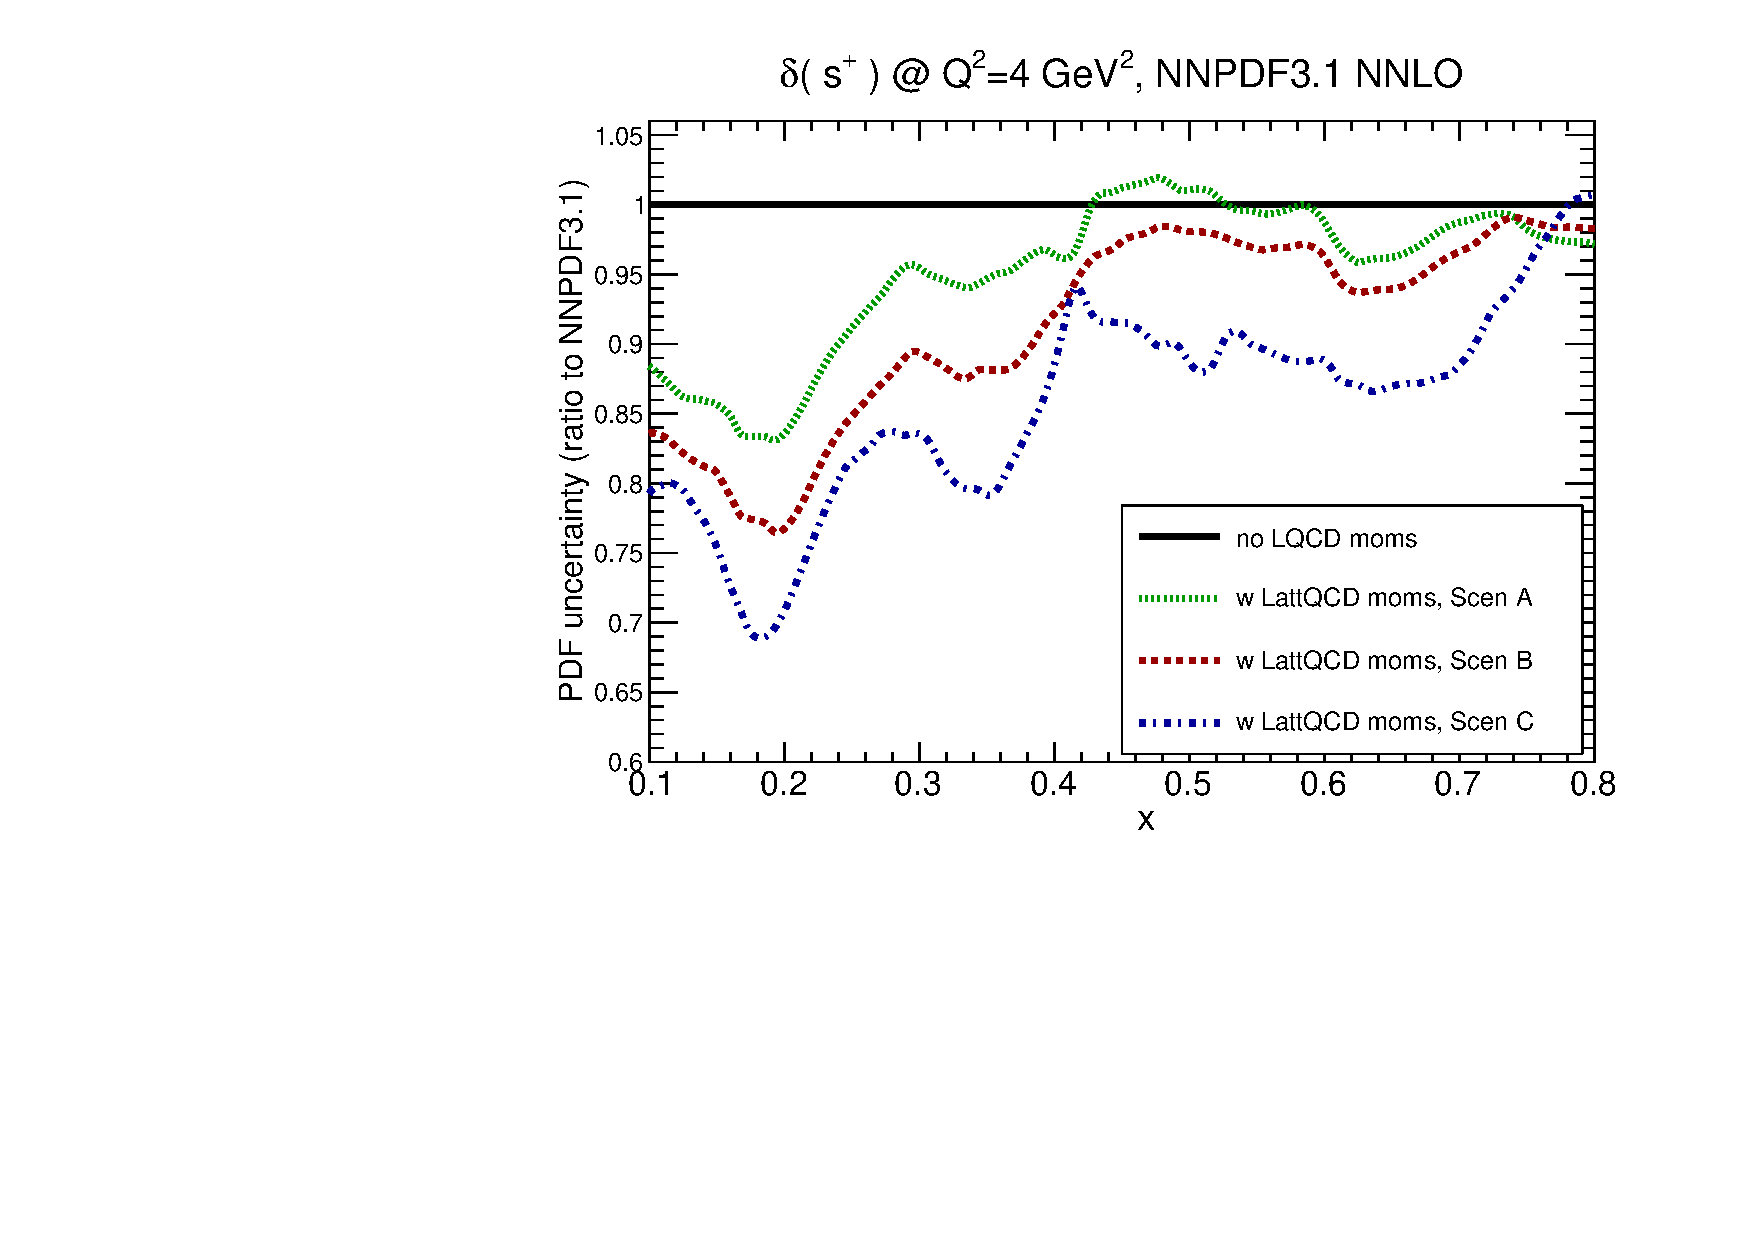
\includegraphics[scale=0.45]{plots/xsp-unpol-lattice-relerr-largex.pdf}
\caption{\small Same as Fig.~\ref{fig:impactUnpol}, now focusing
  on the large-$x$ region, and showing the ratio of the
  PDF uncertainties in the fits based on the three scenarios
  as a ratio of the original
  PDF uncertainty of the NNPDF3.1 NNLO set, for the $d^+$
  and $s^+$ total quark PDFs.
}    
\label{fig:impactUnpollargex}
\end{figure}
%----------------------------------------------------------

\subsubsection*{Impact on polarized global fits}

Next, we move to discuss the results of applying the
reweighting procedure this time to a representative polarized
global fit, specifically the NNPDFpol1.1 NLO set.
%
First of all, in Table~\ref{tab:polmomentsrw}
we list the values of the polarized PDF moments
  used as pseudo-data, as well as the corresponding results
  after the reweighting has been performed for the
three scenarios summarized in 
in Table~\ref{tab:scenarios}.
%
The PDF uncertainties quoted correspond in all cases to 68\%
CL intervals.
%
As we can see from this comparison, already in the first scenario
(which assumes lattice-QCD pseudo-data with similar uncertainties
as existing calculations) there is a marked impact on the
polarized PDF moments.
%
Specifically, for both $\la 1\ra_{\Delta u^+}$ and $\la 1\ra_{\Delta d^+}$
the PDF uncertainties are roughly halved, with the same
trend but less marked for $\la 1\ra_{\Delta s^+}$.
%
At this level, there is no impact for the non-singlet
combinations $\la 1\ra_{\Delta u^+ - \Delta d^+}$
and $\la x\ra_{\Delta u^--\Delta d^-}$.

%%%%%%%%%%%%%%%%%%%%%%%%%%%%%%%%%%%%%%%%%%%%%%%%%%%%%%%%
\begin{table}[t]
  \centering
  \renewcommand{\arraystretch}{1.3} 
\begin{tabular}{c||c||c|c|c}
  \hline &  Original  & Scen A  &  Scen B  & Scen C  \\
  \hline
  $\la 1\ra_{\Delta u^+}$    &  $+0.788\pm  0.079$   & $+0.798\pm  0.039$     &
  $+0.797\pm  0.023$ &   $+0.790\pm  0.009$ \\
  $\la 1\ra_{\Delta d^+}$   &  $-0.450 \pm 0.083$  &  $-0.450 \pm 0.042$  &
  $-0.456 \pm 0.026$    &  $-0.465 \pm 0.012$   \\
  $\la 1\ra_{\Delta s^+}$    &  $-0.124\pm   0.108 $  & $-0.120\pm   0.070 $  &
  $-0.121\pm   0.076 $    &   $-0.111\pm   0.029 $  \\
  $\la 1\ra_{\Delta u^+ - \Delta d^+}$  & $+1.250 \pm 0.024$   & $+1.250 \pm 0.022$  &
  $+1.253 \pm 0.016$ &    $+1.256 \pm 0.012$  \\
  $\la x\ra_{\Delta u^--\Delta d^-}$     & $+0.196 \pm 0.014$    & $+0.195 \pm 0.014$
  & $+0.196 \pm 0.016$     &  $+0.198 \pm 0.012$    \\
  \hline
\end{tabular}
\caption{\small Same as Table~\ref{tab:unpolmomentsrw}, now for
  the polarized PDF moments computed with NNPDFpol1.1.
  %
  The corresponding impact at the PDF level is shown in
  Fig.~\ref{fig:impactPol}.
\label{tab:polmomentsrw}
}
\end{table}
%%%%%%%%%%%%%%%%%%%%%%%%%%%%%%%%%%%%%%%%%%%%%%%%%%%%%%%%

As we further decrease the assumed uncertainties in the lattice-QCD pseudo-data
for the PDF moments, we observe a consequent reduction of the uncertainties
in the global fit.
%
In the most optimistic scenario C, we find that for both
$\la 1\ra_{\Delta u^+}$ and $\la 1\ra_{\Delta d^+}$ there is an uncertainty
reduction by about an order of magnitude as compared to the current values,
and about a factor 5 for $\la 1\ra_{\Delta s^+}$.
%
Therefore, we demonstrate that future lattice-QCD calculations of
polarized PDF moments can potentially lead to a much more
precise understanding of the spin structure of the proton.
%
The other quark combinations exhibit less sensitivity to the inclusion
of the PDF moments in the global fit, given that to begin with
they are already quite well constrained by available experimental
data.
%
Specifically, the PDF uncertainties for  $\la 1\ra_{\Delta u^+ - \Delta d^+}$
are reduced by a factor 2 in this quite optimistic scenario, while
those of $\la x\ra_{\Delta u^--\Delta d^-}$ are essentially unaffected even
in this case.

Next we move to illustrate the impact of the lattice-QCD pseudo-data
on the polarized PDFs themselves, rather than on their
moments.
%
With this motivation,
in Fig.~\ref{fig:impactPol} we present a 
similar comparison as that of Fig.~\ref{fig:impactUnpol}, now
  showing the absolute PDF uncertainties of the NNPDFpol1.1 fit,
  compared to the corresponding results once the lattice pseudo-data
  on polarized moments in included in the analysis by means of the
  reweighting.
  %
  The reason to show absolute rather than relative uncertainties
  is that, unlike unpolarized PDFs, polarized PDFs often exhibit nodes
  (in particular for strangeness and the gluon) and in the nearby regions
  the concept of relative uncertainty becomes ill-defined.
  
%-------------------------------------------------------------------
\begin{figure}[!t]
\centering
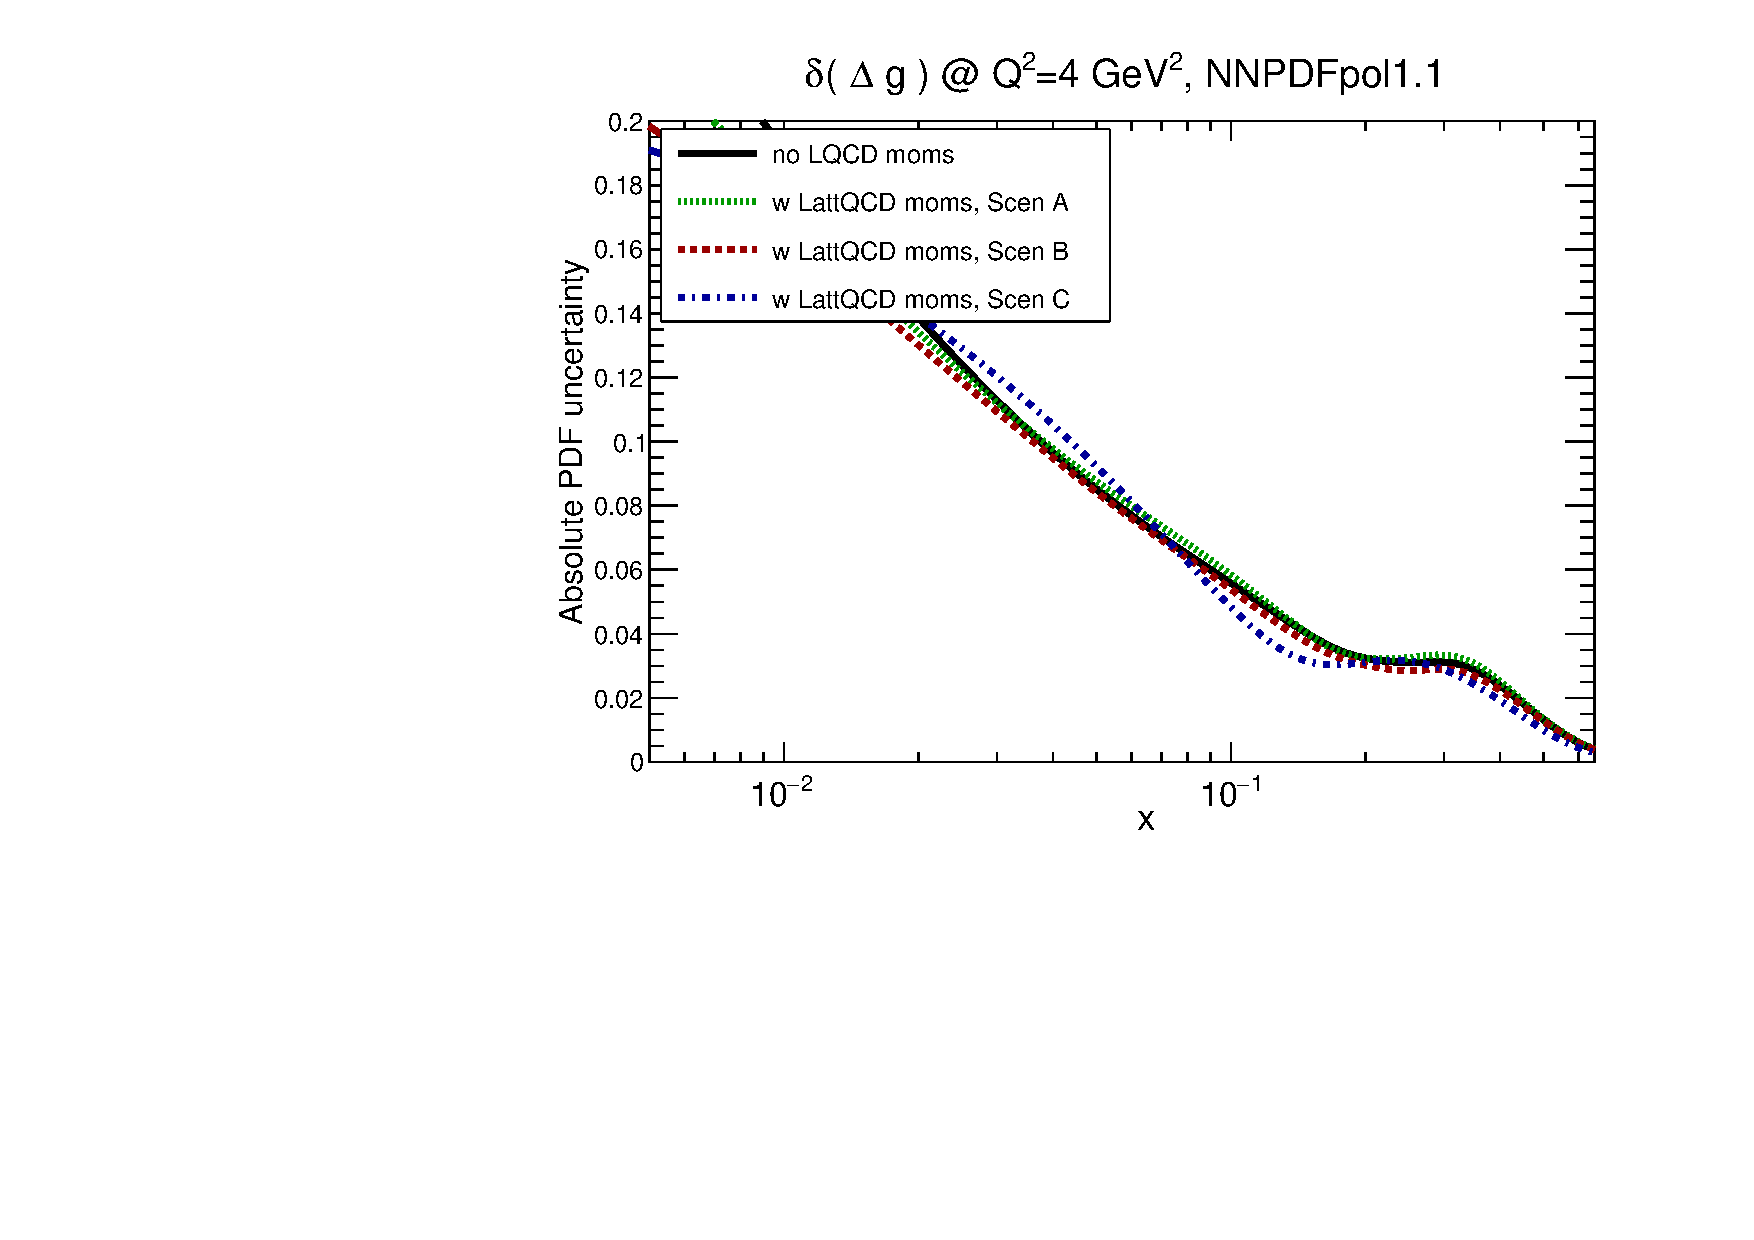
\includegraphics[scale=0.45]{plots/xg-pol-lattice-relerr.pdf}
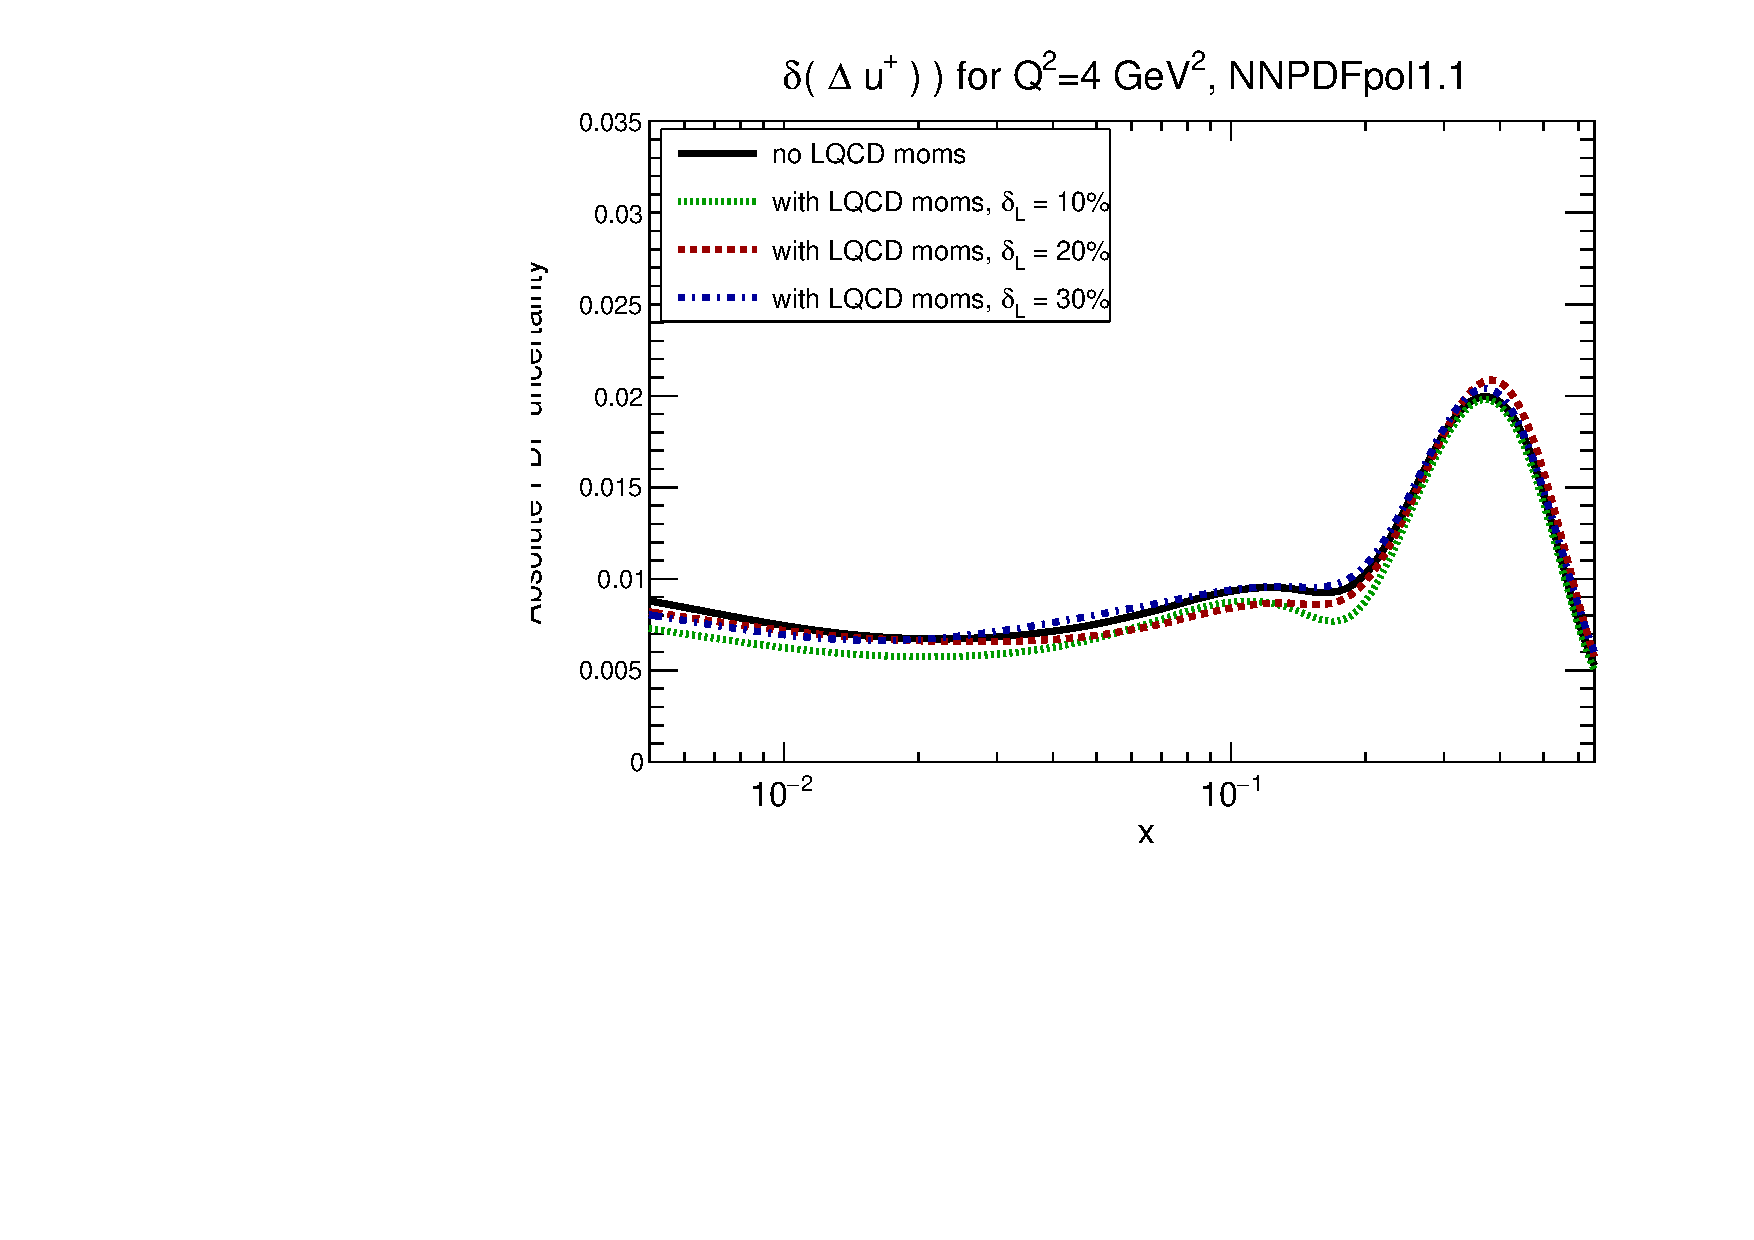
\includegraphics[scale=0.45]{plots/xup-pol-lattice-relerr.pdf}
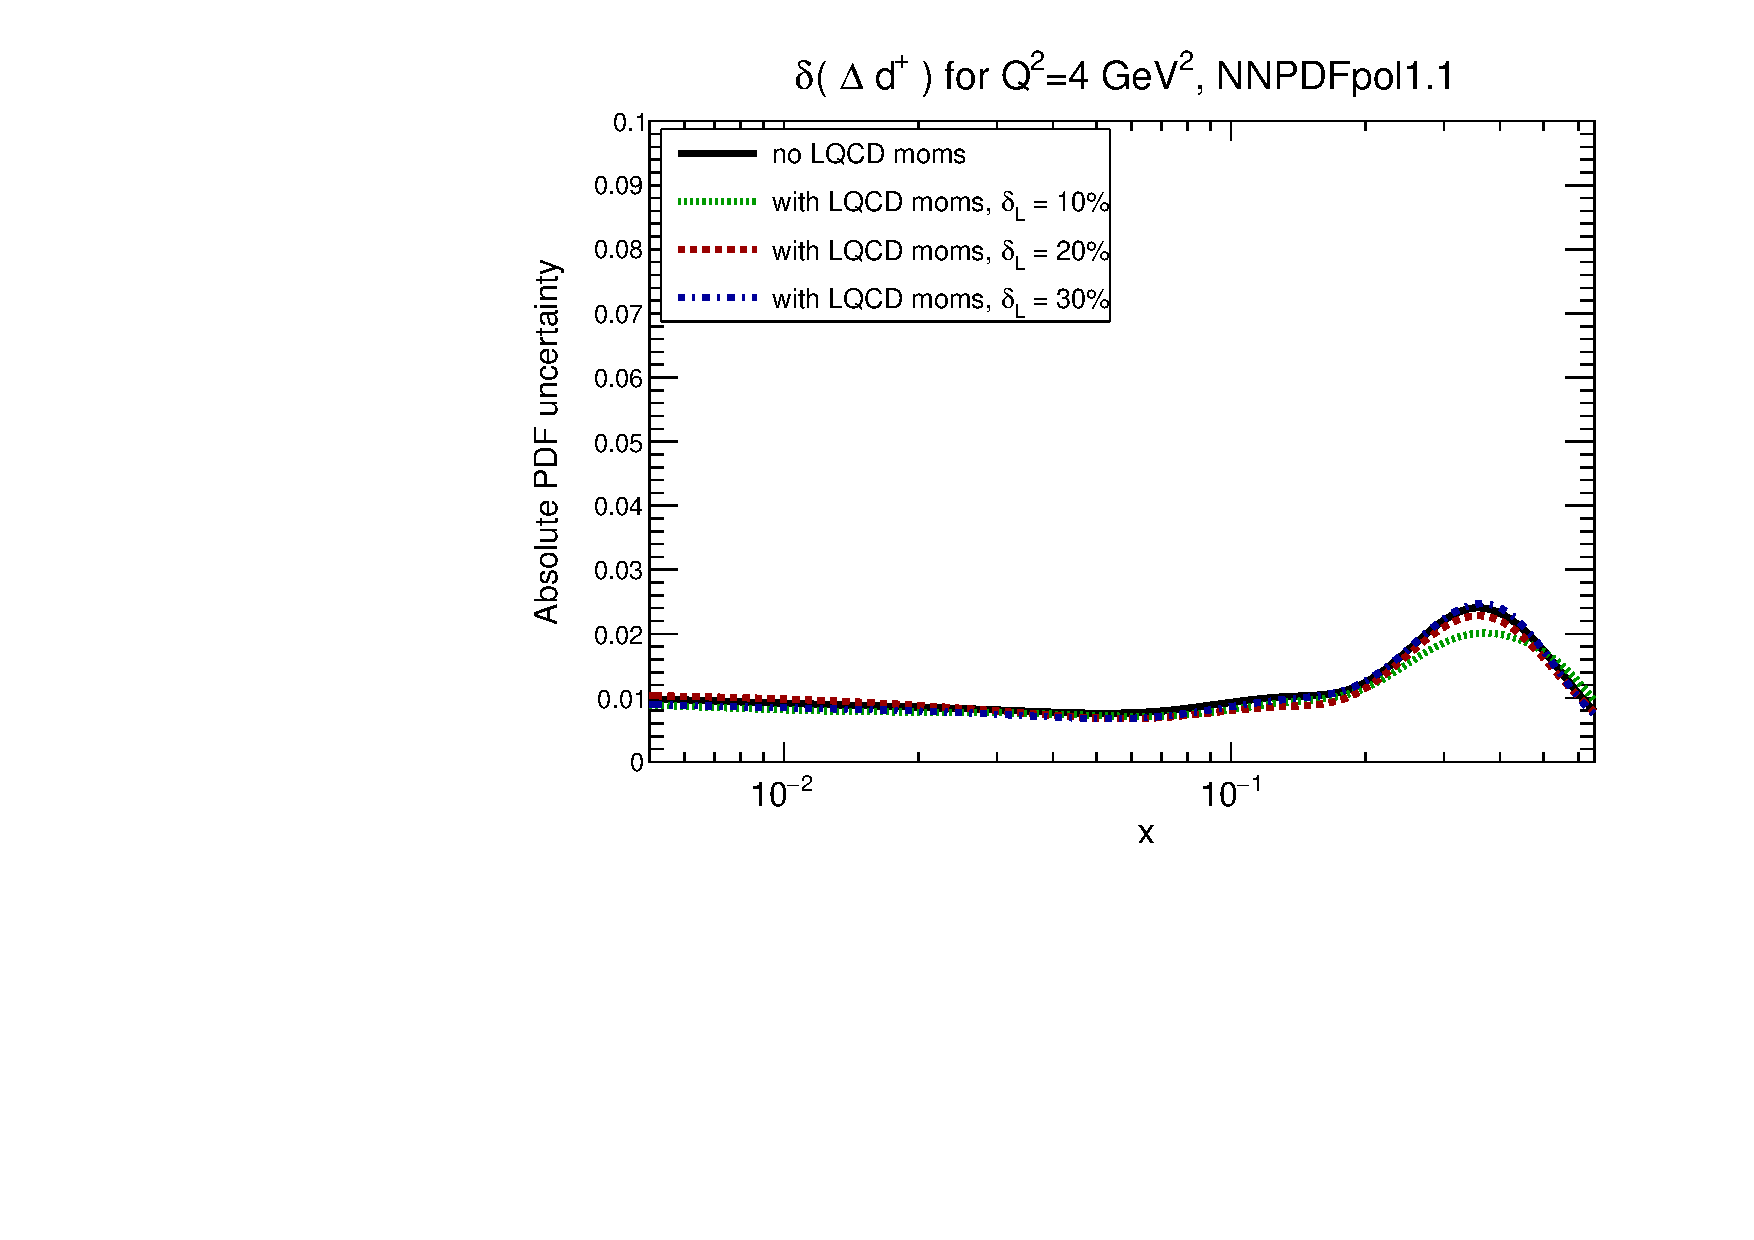
\includegraphics[scale=0.45]{plots/xdp-pol-lattice-relerr.pdf}
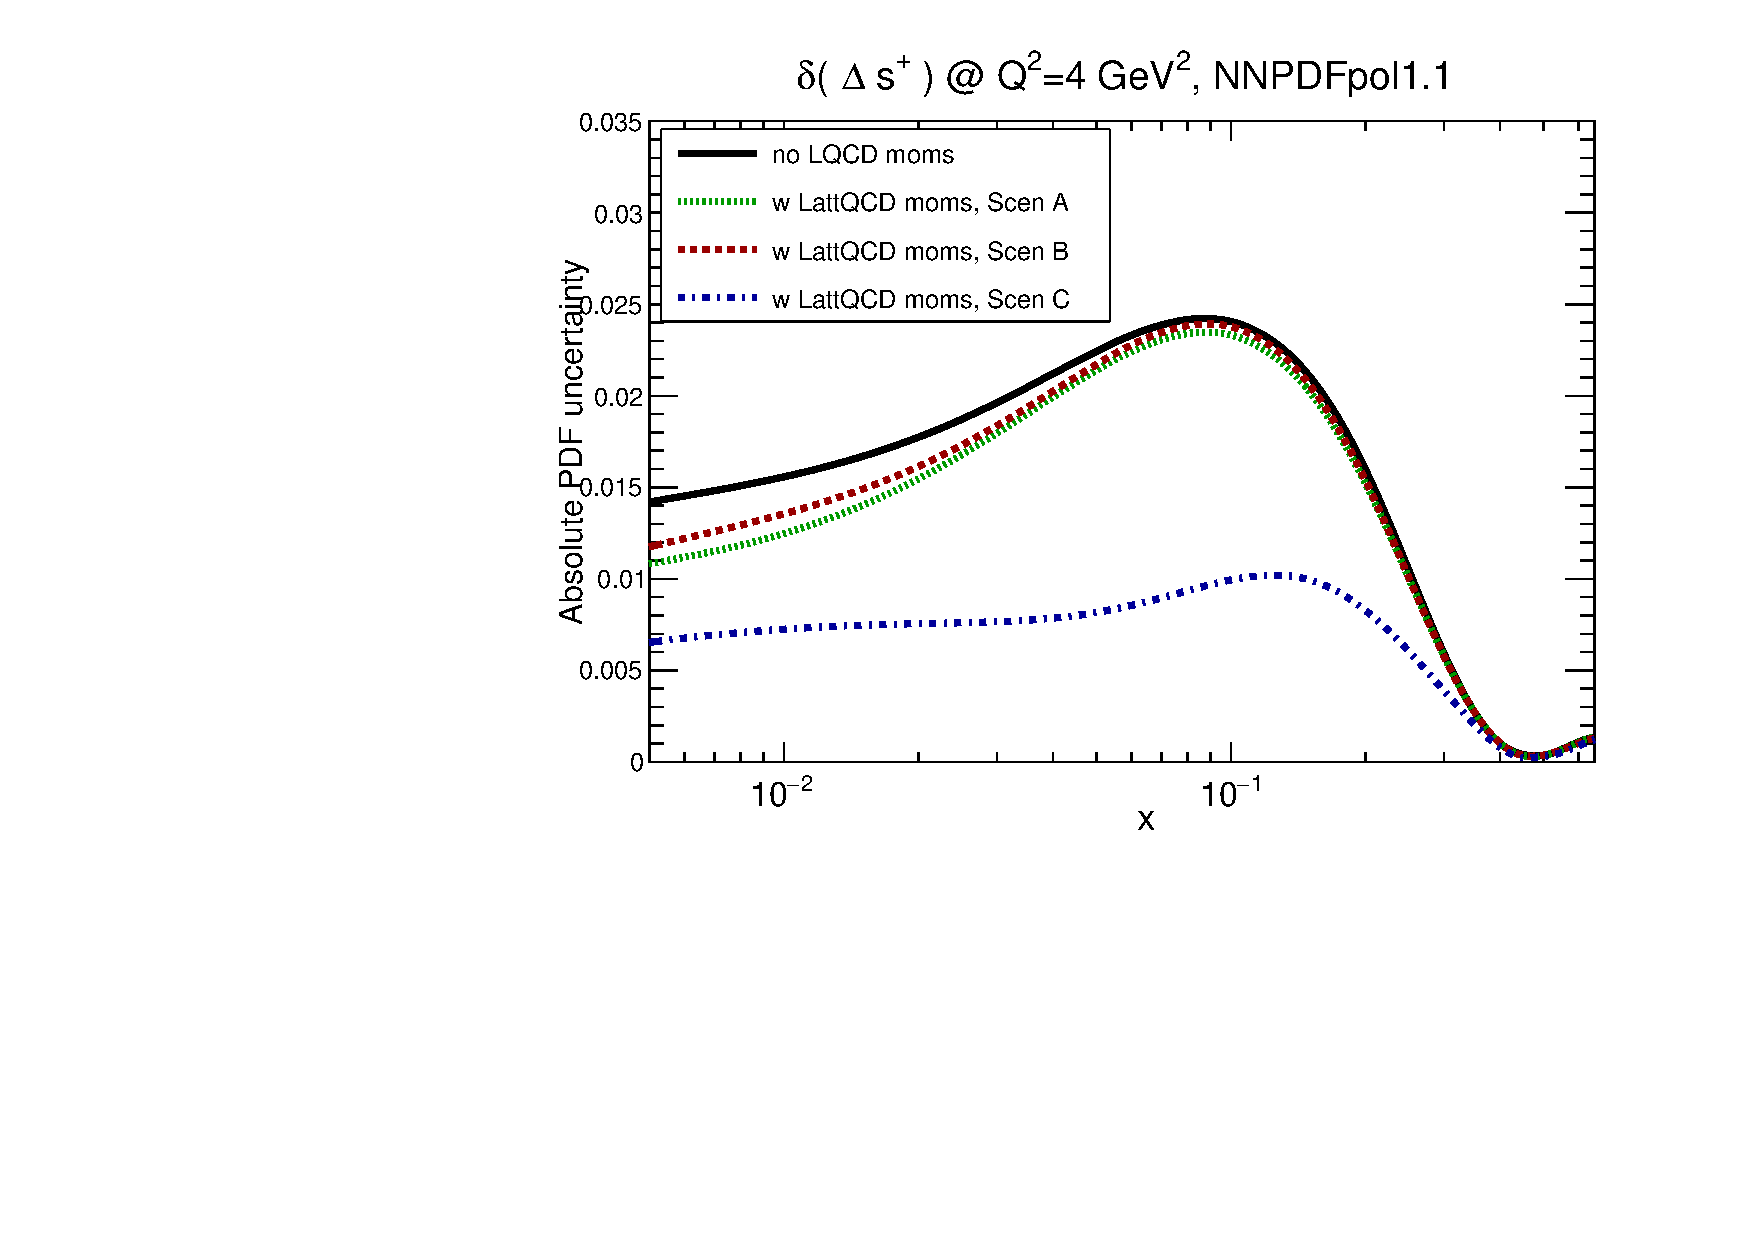
\includegraphics[scale=0.45]{plots/xsp-pol-lattice-relerr.pdf}
\caption{\small Same as Fig.~\ref{fig:impactUnpol}, now
  showing the absolute PDF uncertainties of the NNPDFpol1.1 fit
   $Q^2=4$ GeV$^2$,
  compared to the corresponding results once the lattice pseudo-data
  on polarized moments in included in the analysis via
  reweighting.
}    
\label{fig:impactPol}
\end{figure}
%---------------------------------------------------------------------

From Fig.~\ref{fig:impactPol} we find that for scenarios
A and B there only a very moderate reduction (or even a slight increase)
of the PDF uncertainties, seemingly at odds with the results
for their moments in Table~\ref{tab:polmomentsrw}.
%
The reason is that the first PDF moments alone provide only limited
information on the shape of the PDFs itself, and therefore in some
cases one will find a large error reduction on the moments (since these
are the fitted quantified) than on the PDFs themselves (which are
only directly constrained).
%
On the other hand, once the lattice-QCD pseudo-data uncertainties
decrease beyond a certain level, the start to impact the PDF shape
as well, as we can see from the results of scenario C.
%
In that case we find that the PDF uncertainties can decreases by up to a factor
2 (3) for $\Delta d^+(x,Q)$ ($\Delta s^+(x,Q)$).
%
Interestingly, we see that the relative reduction of PDF uncertainties is more
or less constant along the whole range of $x$, consistent with the fact that
the lattice-QCD pseudo-data is only sensitive to the total integral
of the $x$ distribution.

